\section{Texture mapping}

\subsection{Linear Texture mapping}
The problem solved in this section can be described as follows:
\newline
Given two images, one of a texture and one of a plane, the texture is
mapped onto the plane. 

\begin{figure}[H]
    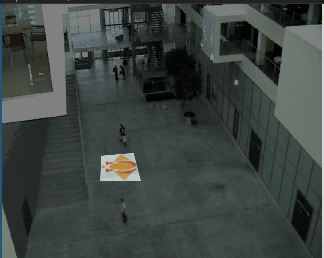
\includegraphics{pics/mapping.png}
    \label{mapping}
\end{figure}

The steps to achieve this are few. 

First, a homography is obtained between the two images though 4 points in each.
These can be selected by the user, or the corners of the image can be used
for the texture. This homography is used to perform a perspective
transform on the texture image with the dimensions of the destination
image. This "warped" image is then used as an overlay on the destination
image. To apply this "overlay" we calculate the weighted sum of the two
arrays (images), the result of this operation is the result image

\subsubsection{Code}
We leverage cv2 to do most of the work here

\begin{verbatim}
    # Grab the homography
    H,Points  = SIGBTools.getHomographyFromMouse(I1,I2,4)
    
    # Dimensions
    h,w,d = I2.shape

    #Perspective transformation
    overlay = cv2.warpPerspective(I1, H,(w, h))

    # Weigthed sum
    M = cv2.addWeighted(I2, 0.5, overlay, 0.5,0)
    
    # Show the image
    cv2.imshow("Overlayed Image",M)

\end{verbatim}

\subsection{Realistic texture mapping}

The problem solved in this section can be described as follows:
\newline
Given two images, one of a texture and one of a plane, the texture is
mapped onto the plane with a single click in the destination image and with
preservation of the textures original dimensions

This problem will be solved through the use of forward mapping and two
homographies.

The steps are as follows

